\documentclass[10]{article}
\usepackage[margin=1in]{geometry}

\usepackage{graphicx}
\graphicspath{{./figs/}}
\usepackage{fancyvrb,color,amssymb,float,alltt,verbatim}
\usepackage{amsmath,mathtools,listings,multicol,hyperref,enumerate}
\usepackage[usenames,dvipsnames,svgnames,table,hyperref]{xcolor}

\usepackage{color}
\usepackage[backend=biber]{biblatex}
\bibliography{final_report}

\begin{document}
\begin{center}
\huge{\textbf{CS229 - Final Report}} \\
\end{center}
\begin{center}
\huge{\textbf{Predicting Political Ideology Using Campaign Finance Data}} \\
\end{center}
\begin{center}
\large{Keri A. McKiernan and Joe A. Napoli \\
\vspace{.25em}
December 12, 2015}
\end{center}
%------------------------------------------------------------------------------%
\section*{Introduction}
% Explain the problem and why it is important. Discuss your motivation for
% pursuing this problem. Give some background if necessary. Clearly state what
% the input and output is. Be very explicit: "The input to our algorithm is an
% {image, amplitude, patient age, rainfall measurements, grayscale video, etc.}.
% We then use a {SVM, neural network, linear regression, etc.} to output a
% predicted {age, stock price, cancer type, music genre, etc.}." This is very
% important since different teams have different inputs/outputs spanning
% different application domains. Being explicit about this makes it easier for
% readers. If you are using your project for multiple classes, add a paragraph
% explaining which components of the project were used for each class.

The public interest has increasingly focused on the effect of money in politics. Specifically, the Citizens United v. FEC Supreme Court ruling maintained the legality of unrestricted political expenditures by corporate and union entities. As a result, there has been a proliferation of super PAC, or `political action committee',  organizations. While these organizations are not permitted to make contributions directly to campaigns, they may engage in unlimited independent spending and there is no restriction on the amount of funds they can accept from donors. Such legal developments beg the question: Can one predict generally the influence of donors over politicians to whom they give? Our project largely builds on previous research conducted by Poole and Rosenthal (summarized below), and makes use of freely available databases of financial information. We aim to predict quantitative scores of political ideology using campaign contribution profiles; specifically, the input to our algorithm is a matrix of normalized vectors of financial data, partitioned by industry, and the output is a score for each candidate on the interval $[-1,1]$ indicating a position on the political ideological spectrum.\\

%------------------------------------------------------------------------------%
\section*{Related Work}
% You should find existing papers, group them into categories based on their
% approaches, and talk about them: Discuss strengths and weaknesses. In your
% opinion, which approaches were clever/good? What is the state-of-the-art? Do
% most people perform the task by hand? You should aim to have at least 5
% references in the related work. Include previous attempts by others at your
% problem, previous technical methods, or previous learning algorithms. Google
% Scholar is very useful for this: https://scholar.google.com/ (you can click
% "cite" and it generates MLA, APA, BibTeX, etc.)

The research of Poole and Rosenthal has focused on quantifying the political ideology of politicians \cite{PR}. In particular, they actively develop methods for calculating `ideal points' of candidates. The DW-NOMINATE method calculates a legislator’s overall probability of voting `yea' on a piece of legislation as the sum of a deterministic utility value and a random error \cite{NOMBOOT}. `Ideal point' coordinates were obtained for legislators by maximizing the log likelihood function

\[ \mathcal{L} = \sum_{t=1}^{T} \sum_{i=1}^{p_t} \sum_{j=1}^{q_t} \sum_{\tau = 1}^{2} C_{ij \tau t} \ln P_{ij \tau t} \]

\noindent where $P_{ij \tau t}$ is the probability of voting for choice $\tau$ (yes or no) and $C_{ij \tau t} = 1$ if that probability accurately predicts the vote \cite{NOMBOOT}. Indexes $j$, $i$, and $t$ sum over roll call votes, legislators, and legislative sessions, respectively. Ideal points are constrained to lie within the interval $\left[ -1,1 \right]$ and are two-dimensional quantities. A common interpretation of the first coordinate is that it reflects the divide between the Republican and Democratic parties, whereas the second coordinate is more highly correlated with intra-party division. While a full congressional voting record would be unavailable for candidates who are new to office, campaign finance data \textit{are} often readily available. It would be useful to be able to predict the ideal point of a candidate even before they have established a congressional voting record. Furthermore, the ability to do so would help elucidate a relationship between monetary contributions to candidates and the voting patterns those contributions may effect.\\

We have collated freely available campaign finance and DW-NOMINATE ideal point \cite{DWWEB} datasets and performed a principal component analysis on the feature set extracted therefrom. The original scope of our project has been narrowed due to a reduction in the size of our group. While originally we had planned to investigate anomalous voting behavior and the ability to predict it solely by examining campaign finance data, we have shifted our focus on training a model to predict DW-NOMINATE ideal points, which directly reflect ideological stances and inter-/intra-party divisions. This shift has been prompted by datasets that were relatively more sparse than expected as well as the challenge of collating them.\\

%------------------------------------------------------------------------------%
\section*{Dataset and Features}
% Give details about your dataset: how many training/validation/test examples do
% you have? Is there any preprocessing you did? What about normalization or data
% augmentation? What is the resolution of your images? How is your time-series
% data discretized? Include a citation to where you got your dataset from.
% Depending on available space, show some examples from your dataset. You should
% also talk about the features you used. If you extracted features using Fourier
% transforms, word2vec, histogram of oriented gradients (HOG), PCA, ICA, etc.
% make sure to talk about it. Try to include examples of your data in the report
% (e.g. include an image, show a waveform, etc.).

\begin{figure}[H]
\centering
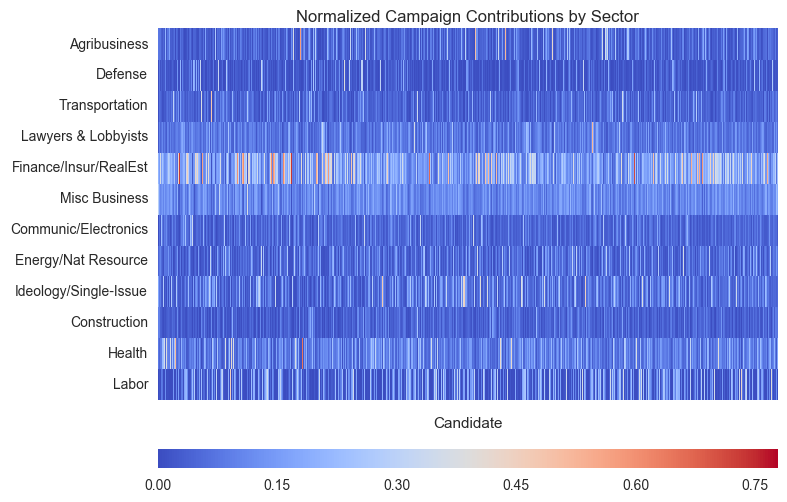
\includegraphics[width=.8\textwidth]{cand_2010_2012_2014_fm_trim_normed_feature_hm.png}
\caption{\label{fig:pc_all}Heatmap of complete feature set}
\end{figure}

%------------------------------------------------------------------------------%
\section*{Methods}
% Describe your learning algorithms, proposed algorithm(s), or theoretical
% proof(s). Make sure to include relevant mathematical notation. For example,
% include the SVM optimization objective/formula or say what the softmax function
% is. It is okay to use formulas from the lecture notes. For each algorithm, give
% a brief description (2-3 sentences) of how it works. Again, we are looking for
% your understanding of how these machine learning algorithms work. Although the
% teaching staff probably know the algorithms, future readers may not (reports
% will be posted on the class website). Additionally, if you are using a niche or
% cutting-edge algorithm (e.g. long short-term memory, SURF features, or anything
% else not covered in the class), you may want to explain your algorithm using
% several paragraphs. Note: Theory/algorithms projects may have an appendix
% showing extended proofs (see appendix description below).

%------------------------------------------------------------------------------%
\section*{Experiments/Results/Discussion}
% You should also give details about what (hyper)parameters you chose (e.g. why
% did you use X learning rate for gradient descent, what was your mini-batch size
% and why) and how you chose them. Did you do cross-validation, if so, how many
% folds? Before you list your results, make sure to list and explain what your
% primary metrics are: accuracy, precision, AUC, etc. Provide equations for the
% metrics if necessary. For results, you want to have a mixture of tables and
% plots. If you are solving a classification problem, you should include a
% confusion matrix or AUC/AUPRC curves. Include performance metrics such as
% precision, recall, and accuracy. For regression problems, state the average
% error. You should have both quantitative and qualitative results. To reiterate,
% you must have both quantitative and qualitative results! This includes
% unsupervised learning (talk with your project TA on how to quantify
% unsupervised methods). Include visualizations of results, heatmaps, examples of
% where your algorithm failed and a discussion of why certain algorithms failed
% or succeeded. In addition, explain whether you think you have overfit to your
% training set and what, if anything, you did to mitigate that. Make sure to
% discuss the figures/tables in your main text throughout this section. Your
% plots should include legends, axis labels, and have font sizes that are
% readable when printed.

We chose a final model after performing a randomized optimization in the space of hyperparameters for SVR, for multiple kernel types. This required specifying distributions over which to sample the hyperparameters. We specified a separate exponential distribution for each hyperparameter, and estimated the decay scale of each distribution by first performing an exhaustive grid search over values of the hyperparameters spanning several orders of magnitude. In both the grid and randomized search schemes, the coefficient of determination ($R^2$) was used as the scoring metric for ranking all sampled models and was estimated for each candidate model using 5-fold cross-validation on a randomly sampled set of training data that comprised 80\% of the data set. Each randomized hyperparameter search proceeded for $30,000$ iterations.\\ 

\begin{center}
\begin{tabular}{ |c|c|c| } 
 \hline
       & \textbf{RBF kernel} & \textbf{Linear kerel} \\ 
 \hline
 C              & 10.77 & 55.33 \\ 
 $\epsilon$     & 0.047 & 0.31 \\
 $\gamma$       & 9.97 & n/a \\
 Training score & 0.82 & 0.70 \\
 Test score     & 0.83 & 0.64 \\
 \hline
\end{tabular}
\end{center}

\noindent The final hyperparameters for the linear and radial basis function (RBF) kernels are summarized in the table below alongside their corresponding training and test errors. We note that results for the polynomial kernel were not as trustworthy because it proved to be much more computationally intensive and thus was unable to be optimized as exhaustively as the other two kernel types. Therefore, we omit those results. We also note that of the best models identified by the randomized search, for each kernel type there were several distinct sets of hyperparameters that yielded very similar training scores. For the RBF kernel specifically, the hypermarameters we selected represent a compromise between the values of C and $\gamma$. While relatively high values of C tend to correspond to overfitting by overpenalizing large deviations from the target, constraining C too aggressively would encourage the bandwidth of the kernel function, $\gamma$, to expand and potentially overfit the data. Therefore, cross-validation will be critical in evaluating the final selection.\\  

\noindent As expected, the RBF kernel is better able to capture the nonlinearities and regional variation of the data by virtue its implicit infinite-dimensional feature mapping. In order to characterize the performance of the final model further as well as to illustrate the deficiencies of the linear kernel, we compute a learning curve of the test score as a function of fraction of data used for training.

\begin{figure}[!htbp]
\begin{center}
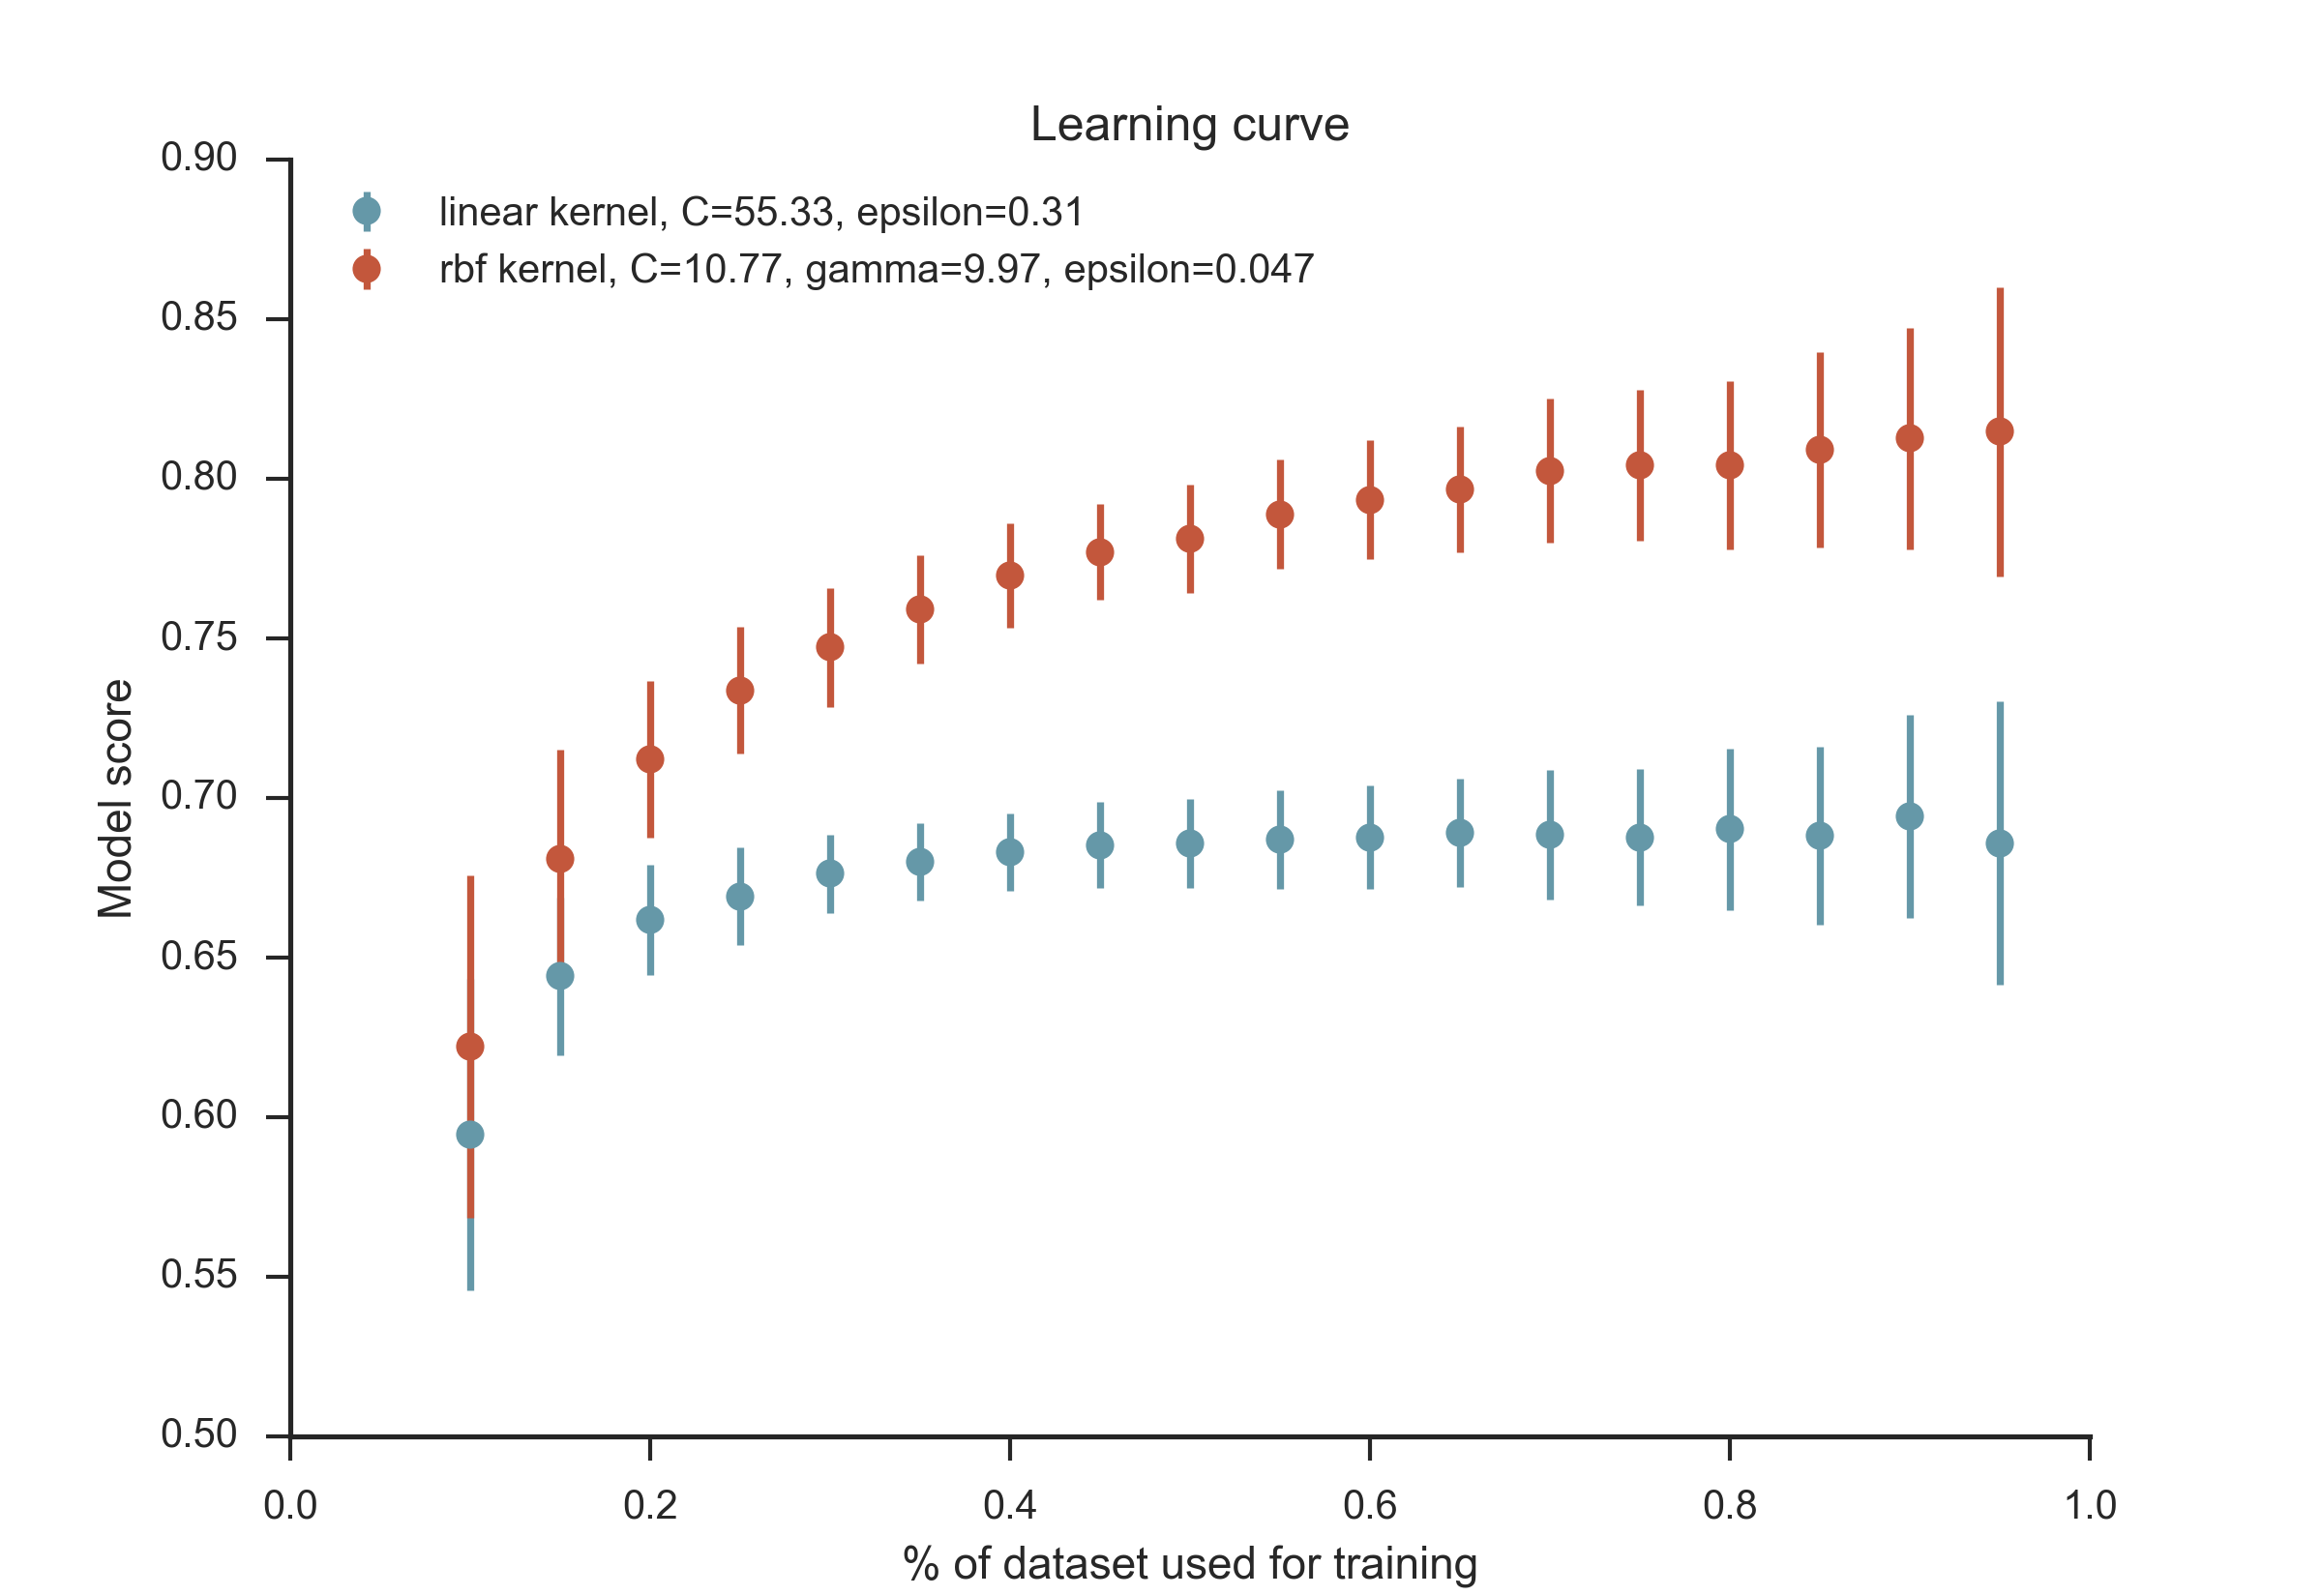
\includegraphics[width=0.8\linewidth]{learning_curve.png}
\caption{Learning curve comparison}
\end{center}
\end{figure}


%------------------------------------------------------------------------------%
\section*{Conclusion/Future Work}
% Summarize your report and reiterate key points. Which algorithms were the
% highest-performing?  Why do you think that some algorithms worked better than
% others? For future work, if you had more time, more team members, or more
% computational resources, what would you explore?

%------------------------------------------------------------------------------%
\end{document}
